\documentclass[twocolumn]{article}
\usepackage{pslatex}
\usepackage{graphicx}

\author{Nick Black\\
\texttt{dankamongmen@acm.org}
\and
Paul Bryan\\
\texttt{paul.bryan@gatech.edu}
}

\title{Implications and Tradeoffs of a\\
Two-Dimensional Mesh Interconnect\\
\small Prepared for CS8803MCA at the Georgia Institute of Technology}

\begin{document}

\maketitle

\pagestyle{headings}

\section{Introduction}

With the advent of widespread multi- and many-core systems, four- and
eight-core processor configurations have become common to the desktop and rack
both. The snooping schemes of broadcast-based shared memories rapidly cease to
scale with even low numbers of processors, reducing the interconnection media
to a chirm of broadcasts and arbitrations and weathering caches with storms of
invalidations. The ubiquitous high-performance MIMD machines of the future, and
today's enterprise-class multiprocessors, will require flexible switched
interconnects to implement their memory hierarchies and facilitate
communication between memories, processors, and memory controllers.

Numerous interconnection methodologies have been suggested, primary among them
the meshes, the \textit{k}-ary \textit{n}-cubes, and the highly indirect Omega,
Delta and Fourier networks. Completion of our distributed memory simulator,
following Project 1's modeling of caches and Project 2's modeling of a
directory for shared memory, necessitated the addition of a switched
interconnect. An incompletely-connected 2-dimensional mesh topology making use
of pipelined switches, dimension-based route selection, and wormhole routing was
implemented. Our simulator supports parameterization of its virtual channel
count, flit length, and virtual channel buffer depth in addition to the
cache parameters of earlier projects.

Choice of a 2-dimensional mesh shaped our results, efforts and design; within
this report, we explore the tradeoffs involved in this interconnection topology
and its underlying properties.

\section{Properties of 2D Meshes}
Two-dimensional meshes are well-suited for current integrated circuit
fabrication technology, as well as Network-on-Chip solutions. Should
three-dimensional fabrication enter the mainstream, their mathematical
properties can be trivially generalized into higher dimensions. The mesh
approach prescribes a quadrilateral (preferably square) geometry, a.k.a. the
\textit{Cartesian planar mesh}; this form minimizes the maximum hop count for a
mesh of $Z$ nodes, where $Z$ is a product of two positive integers $M$ and $N$.
The bandwidth between nodes is typically constant, and has been thus modeled in
our simulator; it is possible that, due to their anisotropic topology (in
contrast with, for instance, a 2D torus), bandwidth might be worth maximizing in
the central lattices and minimizing at the corners\footnote{Random traffic,
assuming a fixed amount of bandwidth available to a Cartesian planar mesh,
would make most efficient use of that bandwidth were it distributed in relation
to a node pair's path distance from the corners.}.

Broadcasting on a mesh is simple, due to the obvious enumerations suggested by
their row-column nature (as opposed to, for instance, a completely connected
interconnect among five nodes (the "full star" topology)), their lack of closed
linear loops (such as those of a torus or ring), and a lack of major
bottlenecks owing to rectilinear symmetry (as opposed to, say, a hierarchal
tree topology). It can be shown that the addition of a single bit to message
headers facilitates broadcasting.

Meshes inherit from their topology properties affecting maximum hop count,
latency, power consumption, bisectional bandwidth, and aggregate bandwidth.
Most striking, at least compared to other methodologies, is the wide variance
between average- and wost-case hop counts, and the resulting spread of
latencies. In the worst case of one corner of the mesh communicating with the
far corner, a full $M+N$ hops must be traversed, assuming no failed nodes along
the path. This maximum hop count might make the mesh topology unusable were it
not for the advent of \textit{wormhole routing} as a successor to the
store-and-forward method; wormhole routing's positive effect upon latency makes
the mesh much more attractive.

Task and data migrations can be employed to bring those processes and data
which generate inter-processor traffic closer together, further reducing the
impact of a mesh's high maximum latency. Furthermore, initial scheduling effecting
localization of communicating processes (and as a secondary weight,
placing isolated processes along the mesh perimeter, where bandwidth is least
dense. The corollary, of course, is to place communicative processes closer
to the central lattice of the mesh, where bandwidth is densest). This
contraindicates a secondary goal of multicore scheduling and migrations, that
of spreading tasks widely across the physical volume with the goal of reducing
local thermal maxima and maximizing contiguous regions suitable for power
saving steps such as sleep states, voltage stepdown or frequency reduction.

Especially due to the performance benefits of localizing schedulers and
migrations, this latter issue seems a reasonable tradeoff. In some
circumstances, however, thermal and electrical properties might carry great
importance. The mesh topology can be adapted to improve delocalized performance,
while retaining some performance benefits, by noting that two different
neighborhoods are at work for each node -- the physical neighborhood, with a
continuous metric specified by the Euclidean distance between nodes (and having as its 
maximum the length of the volume's diagonal), and the
routing neighborhood, with a discrete metric specified by hop count (and having as its
maximum the graph's diameter). The delay introduced by a hop will usually be
substantially greater than that introduced by wiring the corresponding length
alone -- total propagation delay can be expected to remain roughly constant,
while the hop will add processing, queueing, and transmission delay in
proportion to any buffering used. Thus, if deplanarization of the mesh 
and inequality in wire length is not an issue \footnote{For a two dimensional mesh, this means crossing wires; for any number
of dimensions, deplanarization means the maximum distance between two wires of
neighboring nodes will no longer be minimized, as it is in a planar mesh.},
a deplanarized Cartesian mesh could efficiently spread out heat and cut down on
power while adding no new wires\footnote{Longer wires would have negative
impact on propagation delays and required transmission power. If a universal
clock is used, frequency might also be impacted due to longer skew time.}.

Each switch implements a full (local) crossbar; together with the quadrilateral
geometry of the mesh, this results in $Z*2^{O(dimension)}$ links throughout the
interconnect. The extraordinary cost, power and space requirements of crossbars
are well-known, and a full crossbar interconnect would have grown exponentially
with $Z$ (the dimension (here 2) being the base of this exponent). The crossbar-switched
mesh does not, however, bear this heavy monetary cost, growing only linearly
with the addition of nodes. The costs in terms of volume and power, however,
remain, though it is worth noting that nodes can likely be more easily and
precisely powered down than sections of a crossbar fabric, thus allowing for
improvements in power consumption when a system's less than fully utilized.

Meshes are highly resistant to isolated failures, due to a minimum node degree
equivalent to the number of dimensions (it is the corner nodes which suffer
this ignominy). They remain similarly staunch in the face of spherical
volumetric failures, but robustness suffers in proportion to a failure area's
versine and havertangent\footnote{Or increased prolation/oblation of a
failure volume, of course.}. As eccentricity of a large failure volume grows, it may
eventually partition the network, leaving two or more disconnected graphs
incapable of communicating. A fully eccentric (linear) failure spanning the
mesh (ie, a complete row-like or column-like failure) is sufficient to perform
this disconnection\footnote{Formally, a mesh of $D$ dimensions is killed by a
$D-1$-dimensional failure spanning (forming a basis of) the subspace. Thus,
a mesh's robustness is drastically improved with number of dimensions.}

\section{Tradeoffs of 2D Meshes}
The theory of higher-dimensional meshes was explored in Section 2 to depth
suitable for this report; let us now compare meshes, particularly two-dimensional
meshes, to other interconnects. This section assumes planar Cartesian meshes
unless otherwise stated.
\subsection{Meshes and Buses}
A bus (not a circular bus, aka a ring) is merely a singly-dimensional mesh. It
is worth noting that all but antipodal nodes of a bus must be able to transmit
in both directions (corresponding to the $2^O(dimensions)$ of Section 2),
while nodes of a ring could reach all nodes in one direction (with, to be sure,
negative impacts on average and maximum hop counts), representing a cost. In
contrast, a mesh can get by (maintain complete communication) with a minimum of
one link between neighboring rows and columns. This is a special case of Section
2's relation of mesh robustness to dimension. Similarly, failure of any but an
antipodal node immediately bisects a bus\footnote{Polysectionings-at-a-stroke
cannot arise from simultaneous contiguous failure of bus-connected nodes, as
they can in a mesh. This is hardly an argument for buses, but an interesting
point -- decentralization as a robust recovery from failures can be simpler for
buses than meshes.}.

Other comments regarding meshes still apply, especially regarding distribution
along perimeters (poles) and through the central lattice (midsegment). Operating
only in one dimension, and providing only one path between nodes, buses are
very prone to switch stalls. The two-dimensional mesh can be seen as a "sweet
spot" between the performance-starved bus and the complications of three
dimensional meshes.
\subsection{Meshes and Toroids}
Meshes are closely related to toroids in the corresponding number of dimensions,
and their comparison is instructive. Toroids eliminate the border implicit in a
mesh's definition, linking the corresponding nodes of opposite perimeters. The
non-orientable result is the two-dimensional extension of a ring, and has
interesting properties relative to a mesh. Diameter remains $\sqrt(N)$, but the
diameter no longer determines the maximum path length (and thus hop count); a
maximum of $N/2*M/2$ hops need be traversed in an undamaged $N*M$-rectilinear
torus. Bisectional bandwidth is twice that of the mesh, and paths enjoy much
more redundancy (minimum redundancy remains proportional to minimum degree,
which is increased in $D$ dimensions from $D$ to $2^D$.

Toroids are no panacea. Two-dimensional toruses cannot be implemented without
wire crossings in three dimensions\footnote{For analysis of other dimensions,
turn to any topology textbook.}. Toruses of more than one dimension cannot be implemented
without varying wire lengths, and the problems that come with them (see Section 2).

\section{Results and Analysis}
We measured average message latency for several traces, parameterized across
virtual channel count, flit length, and virtual channel buffer depth.
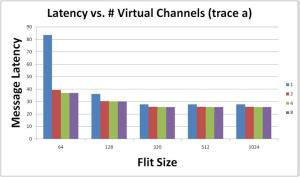
\includegraphics{images/trace_avc_small}
Varying the number of virtual channels had a tremendous impact on average
latency, but only through a pair of channels. Beyond 2, there was little
improvement. Extra virtual channels can only improve performance when messages
are delayed due to contention, corresponding to stalls in the Switch-Allocate
state of our pipelined routers. Were the simulation to lack wormhole routing
or pipelining, extra virtual channels would be much more useful.
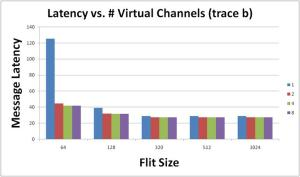
\includegraphics{images/trace_bvc_small}
\newpage
Assuming four virtual channels, flit length and buffer size were varied, and
plotted against average message latency.
\includegraphics{images/traceb_bufsize_small}
Large input buffers are of little advantage in our simulator, due to prolific
use of short (64-bit) messages and a maximum message length of 320 bits. Buffers
of more than 5 flits are a waste of power and hardware.

It's important to note that any hardware element added to the switches or,
worse, to their input buffers will be multiplied across the full interconnect.
While a $4*4$ configuration of virtual channels and input buffers suggests
optimal performance, 2 virtual channels provide almost as much effect for far
lesser total system cost. Our router pipeline saw stalls only in the
Input-Buffer, Virtual-Channel-Allocate and Switch-Allocate stages. These former
only saw stalls due to these parameters, either because no virtual channel was
available or no buffer space was available (as noted, our message sizes meant
that these stalls never occurred in our simulation).

Our traces did not, even in the weakest configurations, saturate the network. It'd
likely be worthwhile to investigate performance at and beyond the saturation point.

\end{document}
